\newpage
\section{Iteración 5: Compensación de posición y trayectoria}

\subsection{Introducción}

Hasta el momento se ha implementado exitosamente un prototipo que se ubica en un mapa gobernado por una red de Petri junto a un Monitor, lo que brinda una representación formal y estructurada del espacio operativo.

En la presente etapa, el objetivo principal es implementar una técnica que permita estimar con precisión la posición del robot dentro de su entorno modelado. Entre las posibles soluciones, se considera la aplicación de un Filtro de Kalman, dada su capacidad para optimizar estimaciones en sistemas dinámicos y con incertidumbre. Este enfoque busca robustecer el desempeño del sistema, incrementando la precisión y confiabilidad en la localización del robot.

\subsection{Requerimientos}

En primer lugar, los requerimientos funcionales a tratar son:

\begin{center} \begin{tabular}{|c|c|} 
\hline
    ID & Descripción \\
\hline
    RF6 & El robot debe recibir y enviar información mediante comunicaciones inalámbricas. \\ 
\hline
    RF8 & Debe poder ubicarse al robot en el plano de forma precisa. \\
\hline
\end{tabular} \end{center}

Por otra parte, los requerimientos no funcionales que abordaremos son:

\begin{center} \begin{tabular}{|p{0.15\linewidth}|p{0.55\linewidth}|} 
\hline
    ID & Descripción \\
\hline
    RNF1 & Debería tener tiempos de respuesta aceptables para el buen funcionamiento del sistema de control. \\
\hline
    RNF2 & El software debería contar con pruebas unitarias y de integración. \\
\hline
    RNF4 & El código debería contar con documentación. \\
\hline
\end{tabular} \end{center}


\subsection{Desarrollo}

\subsubsection{Filtro de Kalman}

El filtro de Kalman es un algoritmo de estimación utilizado para predecir el estado de un sistema dinámico mediante la combinación de datos provenientes de uno o mas sensores, considerando la incertidumbre y el ruido de medición. En el contexto del robot omnidireccional del presente proyecto, este filtro tiene un rol crucial, ya que permite corregir errores en la localización, estimar velocidades más precisas y mejorar la trayectoria mediante la integración de señales provenientes de múltiples sensores.

El funcionamiento del filtro de Kalman se basa en dos etapas: la predicción, donde se estima el próximo estado del sistema utilizando el modelo matemático exacto o teórico; y la actualización, en la que se corrige esa estimación en función de las mediciones actuales, aplicando un modelo probabilístico para minimizar el error. Mediante su modelo probabilístico, es capaz de filtrar el ruido y las imprecisiones de las mediciones, lo que permite obtener una representación confiable del estado.

En cuanto a su implementación, se desarrollará una integración entre el modelo cinemático existente y el filtro de Kalman en Python. Los resultados esperados incluyen un aumento significativo en la precisión de la navegación del robot y una mejora en su capacidad de adaptarse a entornos ruidosos. \cite{negenborn2003robot}


\paragraph{Estimación del estado} \mbox{} \vspace{8pt}

A través de un modelo probabilístico, el filtro combina las predicciones del sistema basadas en el modelo cinemático con mediciones reales provenientes de sensores. Esto permite minimizar el impacto del ruido y las imprecisiones inherentes a las lecturas de los sensores. El proceso de estimación sigue dos etapas principales:

\begin{itemize}
    \item Predicción: Utilizando el modelo de movimiento del robot, se genera una estimación inicial del estado en el instante de tiempo dado.
    \item Actualización: Esta estimación se corrige comparándola con las mediciones obtenidas en tiempo real, ajustando los valores según la incertidumbre de cada fuente de datos. El resultado es una representación más precisa del estado actual del robot.
\end{itemize}

La información estimada por el filtro de Kalman se utiliza para compensar trayectorias y corregir vectores de movimiento. En caso de detectar desviaciones respecto a la trayectoria deseada, se ajustan dinámicamente los comandos de control (distancia y velocidad) enviados al robot, compensando errores como ser resbalamiento, impactos externos e irregularidades del terreno. Esto asegura que el robot mantenga su rumbo previsto con alta precisión y adaptabilidad a entornos variables, además, la capacidad de compensación mejora la fluidez de los desplazamientos.

En términos prácticos, la implementación del filtro de Kalman no solo refuerza la fiabilidad del sistema de navegación, sino que también sienta una base sólida para futuros desarrollos, como la integración con sensores más avanzados o la aplicación en sistemas autónomos.


\paragraph{Matrices de covarianza} \mbox{} \vspace{8pt}

Las matrices de covarianza expresan la relación estadística entre las distintas variables del sistema, cuantificando tanto la magnitud del ruido como la correlación entre las mediciones obtenidas de diferentes sensores. Cada elemento de la matriz de covarianza representa cómo dos variables están relacionadas en términos de su varianza compartida; por lo tanto, si las variables son independientes, sus valores excepto los de la diagonal principal de la matriz son nulos.

El propósito de estas matrices en el filtro de Kalman y en sistemas similares radica en su capacidad para modelar la incertidumbre. Se utilizan tanto en la etapa de predicción, como en la de actualización del filtro para ponderar el impacto de los errores de medición, mejorando las estimaciones del estado. \cite{tzafestas2013introduction} \cite{Rigatos01062007}

La calibración de las matrices de covarianza es crucial para garantizar su correcta representación del ruido real del sistema. Esto puede lograrse mediante técnicas experimentales, analizando mediciones históricas para calcular las varianzas y covarianzas directamente. También se pueden implementar métodos estadísticos que ajusten las matrices iterativamente según los resultados obtenidos durante el funcionamiento del robot. Otra técnica consiste en realizar simulaciones repetitivas, diseñadas para identificar los patrones de error y ajustar las matrices en consecuencia. \cite{Bang18}

\paragraph{Cambio de coordenadas medición/estimación} \mbox{} \vspace{8pt}

Dado que en la próxima iteración se va a colocar una cámara fija en el robot que queremos que esté siempre apuntando hacia el frente, cuando el robot realiza trayectorias y necesita hacer un cambio de dirección, primero realiza un giro sobre su propio eje hasta orientar al robot correctamente.

Por otro lado, el robot al moverse siempre a lo largo sobre su propio eje $y$, va a reportar siempre mediciones donde la velocidad $v_y$ es distinta de cero y $v_x$ es cercana a cero. Es por ello que se agrega una variable que lleva la cuenta de la orientación del robot en grados $[0^{\circ}, 90^{\circ}, 180^{\circ}, 270^{\circ}]$ respecto al sistema de coordenadas global. Con esta información realizamos un cambio de coordenadas para adaptar el sistema de coordenadas locales del robot y sus mediciones, a las globales del mapa.

\paragraph{Implementación} \mbox{} \vspace{8pt}

El filtro de Kalman se implementa de modo que registra velocidad y posición en un eje determinado, por lo que replicando el filtro 2 veces podemos tener una representación de un plano $XY$. Esta implementación se realiza en Python y se integra al funcionamiento del sistema.

Del filtro de Kalman 2D registramos la siguiente tupla:
$$ [x, v_x, y, v_y] $$

Siendo $x$ la posición absoluta en el eje $x$, $v_x$ la velocidad en el eje $x$, $y$ la posición absoluta en el eje $y$ y $v_y$ la velocidad en el eje $y$. Cada Filtro de Kalman se encarga de cada eje $X$ e $Y$ en particular.
Es importante que la entrada y salida del filtro sean del mismo formato, es decir, tenga como entrada y salida la tupla $[x, v_x, y, v_y]$. En este caso introducimos las mediciones acumuladas en distancia y las velocidades en cada eje cartesiano.

La secuencia de procesos a realizar cada vez que se recibe una medición es la siguiente:
\begin{enumerate}
    \item Cálculo del Estado Predicho $X_{kp}$.
    \item Cálculo de la Matriz de Covarianza de Proceso Predicha $P_{kp}$.
    \item Cálculo de la ganancia de Kalman $K$.
    \item Cálculo del Estado Estimado $X_k$.
    \item Actualización de valores.
    \item Actualización de la Matriz de Covarianza de Proceso $P_k$.
\end{enumerate}

Por otra parte, esperamos que el funcionamiento del Filtro de Kalman sea tal que podamos actualizar el estado por cada medición recibida del robot y calcular el vector de compensación según el estado estimado por el filtro. Este proceso se describe en el diagrama de secuencia de la Figura \ref{fig:diagsecuenciafiltrokalman}. \\


\textbf{Adaptación de datos de entrada} \mbox{} \vspace{8pt}

Para comenzar trataremos el proceso para adaptar los datos de las mediciones. En primer lugar, tenemos que el estado observado $Y_k$ puede ser expresado como:

$$ Y_k = C \cdot Y_{km} + Z_k $$

Donde la matriz $C$ transforma la medición al formato necesario, en este caso es una matriz identidad por no necesitar transformarse. Además se tiene la matriz $Z_k$ que modela el error en las observaciones, como ser error en los dispositivos, retardos, fallas mecánicas, entre otras, tambien lo consideramos despreciable.

Por lo que tenemos que el estado observado se puede expresar como:

$$ Y_k =
    \begin{bmatrix}
    1 & 0 \\
    0 & 1  \\
    \end{bmatrix}
    \cdot
    \begin{bmatrix} x_{km} \\ v_{km} \\ \end{bmatrix}
    +
    \begin{bmatrix}
    0 & 0  \\
    0 & 0  \\
    \end{bmatrix}
    =
    \begin{bmatrix} x_{km} \\ v_{km} \\ \end{bmatrix}
$$

Siendo $x_{km}$ y $v_{km}$ los valores de posición y velocidad medidos. La posición es acumulada y la velocidad es la instantánea. \\

\begin{figure}[H]
    \centering
    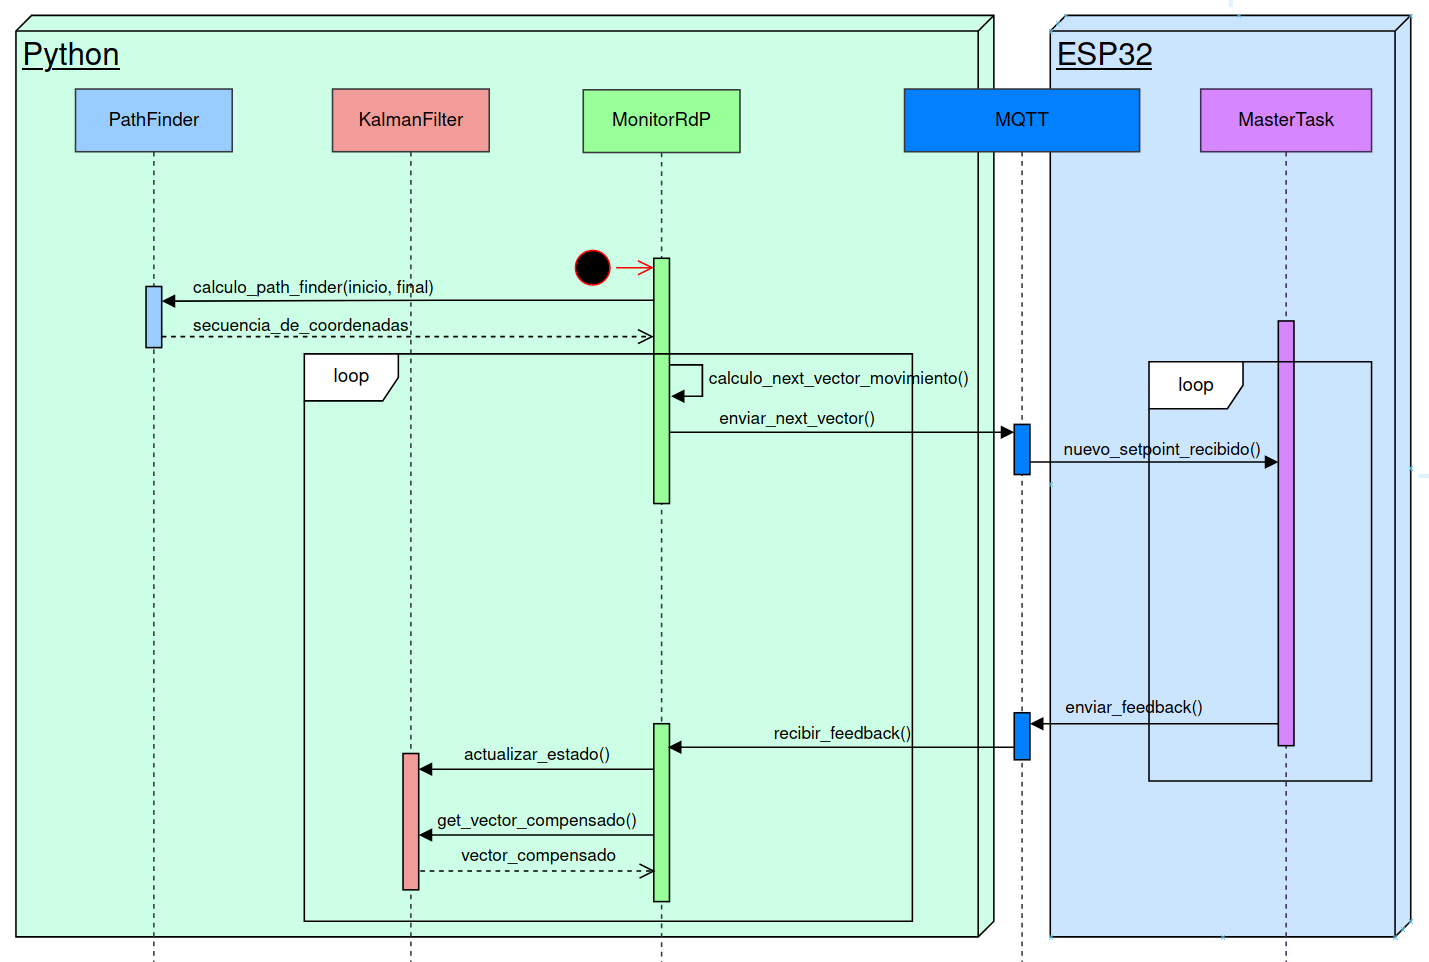
\includegraphics[width=1.1\linewidth]{images/diag_secuencia_filtro_de_kalman_con_esp32.png}
    \caption{Diagrama de secuencia con el Filtro de Kalman}
    \label{fig:diagsecuenciafiltrokalman}
\end{figure}


\textbf{Modelo del filtro} \mbox{} \vspace{8pt}

El filtro de Kalman requiere que modelemos matemáticamente nuestro sistema. En nuestro caso registraremos la posición y velocidad en un eje determinado. El modelo matemático es en base a la ecuación de movimiento rectilíneo acelerado, por lo que para la posición y velocidad instantáneas se tiene:

$$ x = x_0 + x_0 \Delta t + \frac{1}{2} a \Delta t^2 $$
$$ v_x = v_0 + a\Delta t $$

\textbf{Cálculo del Estado Predicho $X_{kp}$} \mbox{} \vspace{8pt}

Este término significa en donde debería estar el robot según el modelo ideal y la distancia entre muestras $\Delta t$. En base a lo anterior en forma matricial, tenemos que el estado predicho está dado por:

$$ X_{kp} =
    \begin{bmatrix} x_{kp} \\ v_{kp} \\ \end{bmatrix}
    =
    A \cdot X_{k-1} + B \cdot U_k + \omega_k
$$

Las matrices A y B representan al modelo en base a las ecuaciones de arriba, mientras que $\omega_k$ representa algún ruido o perturbación presente en el proceso de cálculo del estado predicho. En nuestro caso lo consideramos despreciable, por lo que es nulo. Además, el vector $U_k$ se considera nulo dado que no llevaremos registro de la aceleración del robot.

Donde:

$$
X_{k-1} = \begin{bmatrix} x_{k-1} \\ v_{k-1} \\ \end{bmatrix}
;
A = \begin{bmatrix}
    1 & \Delta t  \\
    0 & 1         \\
    \end{bmatrix} \\
;
B = \begin{bmatrix}
    \frac{1}{2} \Delta t^2 \\
    \Delta t               \\
    \end{bmatrix}          \\
;
U_k = \begin{bmatrix} a_0 \\ \end{bmatrix} \\
;
\omega_k = \begin{bmatrix} 0 \\ 0 \\ \end{bmatrix}
$$

Entonces la ecuación para obtener el nuevo estado predicho:

$$
X_{kp} = 
    \begin{bmatrix}
    1 & \Delta t  \\
    0 & 1         \\
    \end{bmatrix} \\
    \cdot \begin{bmatrix} x_{k-1} \\ v_{k-1} \\ \end{bmatrix}
    +
    \begin{bmatrix}
    \frac{1}{2} \Delta t^2 \\
    \Delta t               \\
    \end{bmatrix}          \\
    \cdot
    \begin{bmatrix} 0 \\ \end{bmatrix} \\
    +
    \begin{bmatrix} 0 \\ 0 \\ \end{bmatrix}
$$ \\

\textbf{Cálculo de Matriz de Covarianza de Proceso Predicha $P_{kp}$} \mbox{} \vspace{8pt}

Esta matriz se modela teniendo por un lado el término $\Delta_{px}$ y por otro lado el término $\Delta_{pv_x}$ que representan errores en el proceso de calcular la posición y velocidad predichos.

En el caso que exista relación en la incerteza del proceso para calcular la posición y velocidad, el término $\Delta_{px} \cdot \Delta_{pv_x}$ es distinto de cero. En nuestro caso lo establecemos en $0$.

Por lo que se tiene la siguiente matriz de covarianza inicial:

$$
P_{k-1} = \begin{bmatrix}
    {\Delta_{px}}^2 & \Delta_{px} \cdot \Delta_{pv_x} \\
    \Delta_{px} \cdot \Delta_{pv_x} & {\Delta_{pv_x}}^2 \\
    \end{bmatrix} \\
    = \begin{bmatrix}
    {\Delta_{px}}^2 & 0 \\
    0 & {\Delta_{pv_x}}^2 \\
    \end{bmatrix} 
$$

Luego, para calcular la nueva matriz se parte de la siguiente expresión:

$$ P_{kp} = A \cdot P_{k-1} A^T + Q_k $$

Donde la matriz A es la misma expresada en el paso anterior y $Q_k$ modela el error en el proceso de cálculo de las matrices de covarianza, también establecido en $0$. Por lo que obtenemos:

$$ P_{kp} =
    \begin{bmatrix}
    1 & \Delta t  \\
    0 & 1         \\
    \end{bmatrix} \\
    \cdot 
    \begin{bmatrix}
    {\Delta_{px}}^2 & 0   \\
    0 & {\Delta_{pv_x}}^2 \\
    \end{bmatrix}
    \cdot
    \begin{bmatrix}
    1 & 0           \\
    \Delta t & 1    \\
    \end{bmatrix}   \\
    +
    \begin{bmatrix}
    0 & 0  \\
    0 & 0  \\
    \end{bmatrix}  \\
$$

\textbf{Cálculo de la ganancia de Kalman $K$} \mbox{} \vspace{8pt}

La ganancia de Kalman en pocas palabras es una media ponderada que le da mas o menos importancia a la medición versus la estimación según el error detectado. Si la ganancia $K$ tiende a 0, indica que el sistema no converge y que tiene un error considerable. Por otro lado si la ganancia $K$ tiende a 1 indica que tiene poco error.

Para calcular la ganancia de Kalman utilizamos la siguiente expresión:

$$ K = \frac{P_{kp} \cdot H^T}
            {H \cdot P_{kp} \cdot H^T + R}
$$

Donde la matriz $H$ es una matriz identidad $I$ que se utiliza para convertir el dominio de los datos al formato que necesita $K$. La matriz $R$ es una matriz de covarianzas que representa los errores en la observación, que se puede simplificar del mismo modo que $P_{kp}$ y se puede expresar como:

 $$ R =
    \begin{bmatrix}
    {\Delta_x}^2 & \Delta_x \cdot \Delta_{v_x} \\
    \Delta_x \cdot \Delta_{v_x} & {\Delta_{v_x}}^2 \\
    \end{bmatrix} \\ 
    =
    \begin{bmatrix}
    {\Delta_x}^2 & 0 \\
    0 & {\Delta_{v_x}}^2 \\
    \end{bmatrix} \\ 
$$

Por lo que para calcular la ganancia de Kalman:

$$ K =
    \frac{
        \begin{bmatrix}
        {\Delta_{px}}^2 & 0 \\
        0 & {\Delta_{pv_x}}^2 \\
        \end{bmatrix}
        \cdot
        \begin{bmatrix}
        1 & 0 \\
        0 & 1  \\
        \end{bmatrix}
        }
    {
        \begin{bmatrix}
        1 & 0 \\
        0 & 1  \\
        \end{bmatrix}
        \cdot
        \begin{bmatrix}
        {\Delta_{px}}^2 & 0 \\
        0 & {\Delta_{pv_x}}^2 \\
        \end{bmatrix}
        \cdot
        \begin{bmatrix}
        1 & 0 \\
        0 & 1  \\
        \end{bmatrix}
        +
        \begin{bmatrix}
        {\Delta_x}^2 & 0 \\
        0 & {\Delta_{v_x}}^2 \\
        \end{bmatrix} \\ 
    }
$$ \\

\textbf{Cálculo del Estado Estimado $X_k$} \mbox{} \vspace{8pt}

Para obtener la nueva estimación del estado en base a la última medición recibida, podemos expresar:

$$ X_k = X_{kp} + K \cdot ( Y_k - H \cdot X_{kp} ) $$

Donde $X_{kp}$ es el estado predecido, $K$ es la ganancia de Kalman, $Y_k$ es la medición observada y $H$ una matriz de conversión. Esta ultima resulta ser una matriz identidad por no ser necesario convertir los datos del estado predicho.

$$ X_k =
    X_{kp}
    +
    K
    \cdot (
        \begin{bmatrix} x_{km} \\ v_{km} \\ \end{bmatrix}
        -
        \begin{bmatrix}
        1 & 0 \\
        0 & 1  \\
        \end{bmatrix}
        \cdot
        X_{kp}
    )
$$ \\

\textbf{Actualización de la Matriz de Covarianza de Proceso $P_k$} \mbox{} \vspace{8pt}

Eventualmente, cuando el error se reduce lo suficiente, podemos actualizar la matriz de covarianza de proceso mediante la siguiente expresión:

$$ P_k = ( I - K \cdot H ) \cdot P_{kp} $$

Donde $H$ nuevamente es una matriz identidad. Por lo que resulta:

$$ P_k =
    (
    \begin{bmatrix}
    1 & 0 \\
    0 & 1  \\
    \end{bmatrix}
    -
    K
    \cdot
    \begin{bmatrix}
    1 & 0 \\
    0 & 1  \\
    \end{bmatrix}
    )
    \cdot
    P_{kp}
$$

\textbf{Actualización de valores} \mbox{} \vspace{8pt}

Antes de comenzar una nueva iteración debemos actualizar los valores de la matriz de covarianza y la de estado predecido:

$$ P_{k-1} = P_k $$
$$ X_{k-1} = X_k $$

\subsubsection{Compensación con Filtro de Kalman}

Dado que el filtro de Kalman puede estimar con precisión un estado en base a sucesivas mediciones, podemos utilizarlo para ubicar en todo momento al robot en el plano con su coordenada y velocidad estimadas. Esta información la podemos utilizar para determinar la corrección necesaria a aplicar para que el robot corrija su trayectoria, procederemos a describir este proceso.

Vale aclarar que el robot recibe comandos del siguiente formato, donde se especifica la distancia a recorrer con un vector determinado:
$$ [distancia, v_x, v_y, v_\theta] $$

Por otra parte el robot reporta el feedback de modo que es apto para el filtro de Kalman:
$$ [x, v_x, y, v_y] $$

\paragraph{Compensación espacial y vectorial} \mbox{} \vspace{8pt}

La compensación espacial y vectorial del robot omnidireccional se logra aprovechando las capacidades del filtro de Kalman para estimar el estado actual del sistema en tiempo real. Con esta información, el sistema puede ajustar los vectores de movimiento en las ruedas, compensando automáticamente irregularidades en el desplazamiento.

La corrección de la \textit{posición} del robot se realiza principalmente a través del filtro de Kalman, que combina el modelo cinemático con las mediciones reales para determinar en todo momento la ubicación exacta del robot en el espacio y su velocidad. Cuando se detectan desviaciones en la posición estimada, el filtro ajusta la estimación para reducir el error acumulado y garantizar un control óptimo.

Por otro lado, la \textit{trayectoria} planeada se corrige utilizando el modelo cinemático del robot. Este modelo define las relaciones entre los vectores de movimiento de las ruedas y los desplazamientos deseados en el espacio. Cuando el filtro de Kalman detecta desviaciones en la posición real, el sistema utiliza esta información para recalcular y corregir la trayectoria, asegurando que el robot siga el camino previamente definido.

\paragraph{Implementación} \mbox{} \vspace{8pt}

\textbf{Compensación espacial} \mbox{} \vspace{8pt}

Para la compensación espacial necesitamos determinar $d_c$, que es la distancia a recorrer para corregir la posición y llegar a $B$.

Definimos la compensación para un desplazamiento en el eye $y$ del mapa, luego se comprueba que el proceso es el mismo para un desplazamiento en $x$. En primer lugar se definen tres puntos claves:

$$ A = (x_1, y_1) : \text{Punto de partida} $$
$$ B = (x_2, y_2) : \text{Punto de llegada} $$
$$ X_a = (x_a, y_a) : \text{Coordenada actual del robot estimada por Kalman} $$
$$ d_c = (d_{xc}, d_{yc}) : \text{Distancia de compensación} $$

\begin{figure}[H]
    \centering
    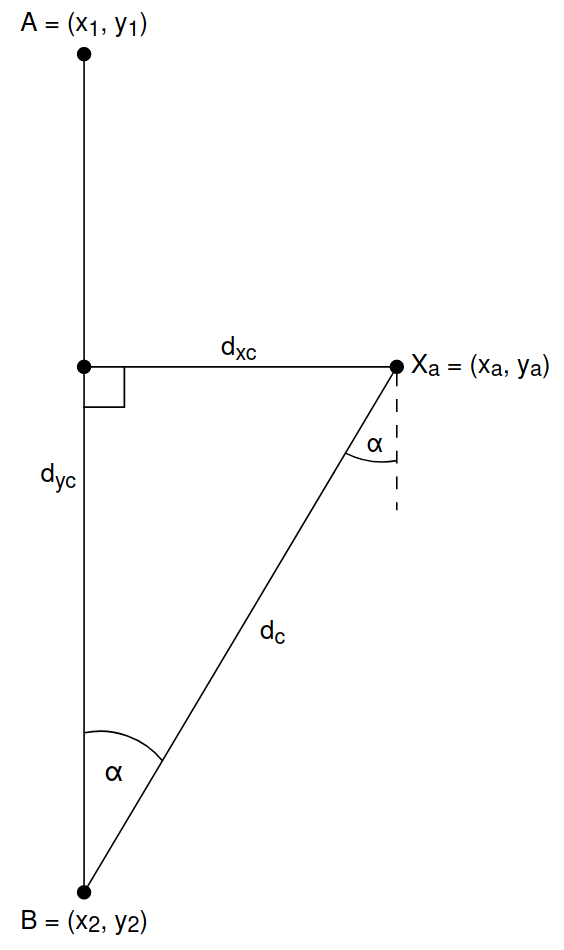
\includegraphics[width=0.4\linewidth]{images/compensacion_vector_distancia_kalman.png}
    \caption{Diagrama de compensación espacial}
    \label{fig:diagcompespacial}
\end{figure}

Para ello podemos definir:

$$ d_c = \sqrt{ {d_{xc}}^2 + {d_{yc}}^2 } $$
$$ d_{xc} = x_2 - x_a $$
$$ d_{yc} = y_2 - y_a $$

Con lo que podemos calcular $d_c$ para completar la tupla enviada al robot.

Ahora bien, en este punto podemos obtener el valor de $\alpha$:

$$ tan(\alpha) = \frac{d_{xc}}{d_{yc}} $$
$$ \alpha = arctan(\frac{d_{xc}}{d_{yc}}) $$

Es posible comprobar que para un desplazamiento sobre el eje $x$, la diferencia es que se calcula $\alpha$ de la siguiente manera:

$$ \alpha = arctan(\frac{d_{yc}}{d_{xc}}) $$

\textbf{Compensación vectorial} \mbox{} \vspace{8pt}

Para la compensación vectorial, en primera instancia definimos:

$$ V_c = (V_{xc}, V_{yc}) : \text{Vector de compensación} $$

\begin{figure}[H]
    \centering
    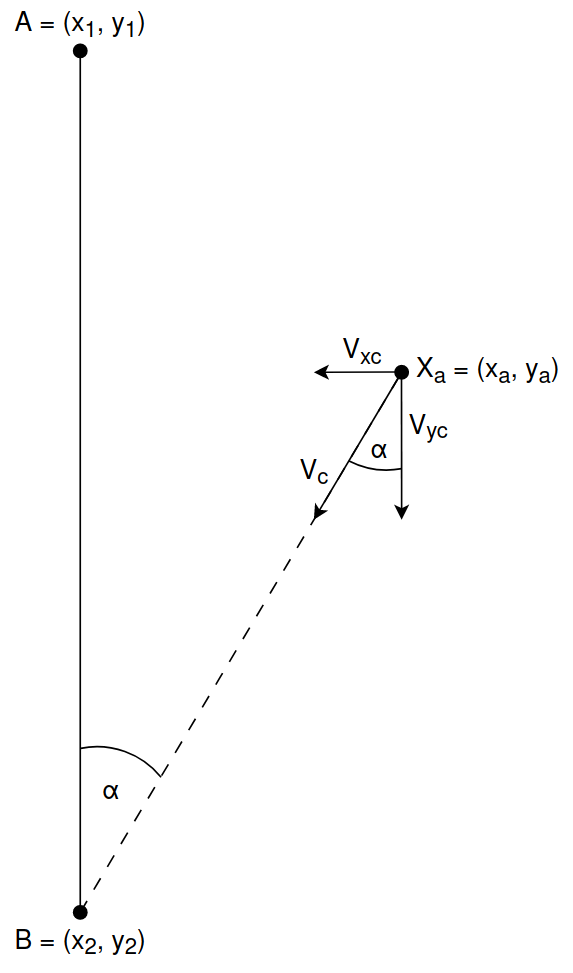
\includegraphics[width=0.4\linewidth]{images/compensacion_vector_velocidad_kalman.png}
    \caption{Diagrama de compensación vectorial}
    \label{fig:diagcompvectorial}
\end{figure}

Ahora bien, se establece que el valor de velocidad de compensación $V_c$ es constante, pero aún así necesitamos descomponer el vector para obtener $V_{xc}$ y $V_{yc}$ para enviarlo al robot:

$$ V_{xc} = V_c \cdot sen(\alpha) $$
$$ V_{yc} = V_c \cdot cos(\alpha) $$

Por lo que podemos definir:

$$ tan(\alpha) = \frac{V_{xc}}{V_{yc}} $$
$$ \alpha = arctan(\frac{V_{xc}}{V_{yc}}) $$

Con lo que ya podemos calcular $V_{xc}$ y $V_{yc}$ para enviarlo en la tupla que recibe el robot. En las tuplas del vector de compensación $v_\theta = 0$ dado que nuestro modelo de Kalman no contempla desplazamiento rotacional.

Es posible comprobar que para un desplazamiento sobre el eje $x$, la diferencia es que calculamos $\alpha$ de la siguiente manera:

$$ \alpha = arctan(\frac{V_{yc}}{V_{xc}}) $$

\subsection{Testing y pruebas}

Todas las pruebas realizadas en esta iteración parten del desarrollo realizado hasta el momento del prototipo, la interfaz y el modelo del mapa.

\begin{testtableformat}
    \hline \rowcolor{test_header_color}
        Test ID             & TC\_05\_00 \\
    \hline
        Tipo de test        & Test unitario \\
    \hline
        Objeto de prueba    & Filtro de Kalman \\
    \hline
        Requerimiento       & RF8 - RF6 \\
    \hline
        Nombre              & Estimación del Filtro de Kalman \\
    \hline
        Descripción         & Determinar la estimación del Filtro de Kalman luego de N iteraciones de mediciones, con trayectorias en linea recta sin cambio de dirección \\
    \hline
        Precondición        & PRECOND\_H \\
    \hline
        Pasos del test      & \begin{enumerate}
                                \item Enviar al robot setpoints en linea recta y recolectar las mediciones
                                \item Introducir las mediciones en el Filtro de Kalman y verificar que la estimación realizada se condice con la posición real final del robot
                                \item Repetir desde el paso 1) con diferentes valores
                            \end{enumerate} \\
    \hline
        Resultado esperado  & La estimación hecha por el Filtro de Kalman luego de N iteraciones debe aproximarse a la coordenada real del robot en el espacio \\
    \hline
        Resultado obtenido  & Se obtiene que la estimación de Kalman es correcta con un error de alrededor de $\pm3[cm]$ \\
    \hline
        Observaciones       & - \\
    \hline
\end{testtableformat}


\begin{testtableformat}
    \hline \rowcolor{test_header_color}
        Test ID             & TC\_05\_01 \\
    \hline
        Tipo de test        & Test unitario \\
    \hline
        Objeto de prueba    & Filtro de Kalman \\
    \hline
        Requerimiento       & RF8 - RF6 \\
    \hline
        Nombre              & Estimación del Filtro de Kalman \\
    \hline
        Descripción         & Determinar la estimación del Filtro de Kalman luego de N iteraciones de mediciones, con trayectorias en linea recta con cambio de dirección respetando la restricción de movimiento \\
    \hline
        Precondición        & PRECOND\_H \\
    \hline
        Pasos del test      & \begin{enumerate}
                                \item Enviar al robot setpoints en linea recta con cambios de dirección y recolectar las mediciones
                                \item Introducir las mediciones en el Filtro de Kalman y verificar que la estimación realizada se condice con la posición real final del robot
                                \item Repetir desde el paso 1) con diferentes valores
                            \end{enumerate} \\
    \hline
        Resultado esperado  & La estimación hecha por el Filtro de Kalman luego de N iteraciones debe aproximarse a la coordenada real del robot en el espacio \\
    \hline
        Resultado obtenido  & Se obtiene que la estimación de Kalman se aproxima a la real con un radio de $\pm3[cm]$ en las coordenadas XY \\
    \hline
        Observaciones       & - \\
    \hline
\end{testtableformat}


\begin{testtableformat}
    \hline \rowcolor{test_header_color}
        Test ID             & TC\_05\_02 \\
    \hline
        Tipo de test        & Test de integración \\
    \hline
        Objeto de prueba    & Compensador del Filtro de Kalman \\
    \hline
        Requerimiento       & RF8 - RF6 - RF5 - RF3 \\
    \hline
        Nombre              & Compensación del Filtro de Kalman apagada \\
    \hline
        Descripción         & Se debe tomar un punto de referencia sobre el cual comparar la acción de la compensación del filtro. Realizar compensaciones en base a las mediciones acumuladas sin ser procesadas por el filtro. Se realizan los experimentos con trayectorias en línea recta sin cambio de dirección \\
    \hline
        Precondición        & PRECOND\_G \\
    \hline
        Pasos del test      & \begin{enumerate}
                                \item Enviar al robot setpoints en linea recta y recolectar las mediciones
                                \item Calcular compensaciones sin utilizar el Filtro de Kalman y comprobar la posición final del robot
                                \item Repetir desde el paso 1) con diferentes valores
                            \end{enumerate} \\
    \hline
        Resultado esperado  & El robot debe lograr llegar a destino con un comportamiento similar al obtenido con las pruebas del Modelo Cinemático en línea recta, con su error asociado \\
    \hline
        Resultado obtenido  & Al realizar la trayectoria se observan desviaciones considerables, comparables a las pruebas solo con Modelo Cinemático compensado \\
    \hline
        Observaciones       & - \\
    \hline
\end{testtableformat}


\begin{testtableformat}
    \hline \rowcolor{test_header_color}
        Test ID             & TC\_05\_03 \\
    \hline
        Tipo de test        & Test de integración \\
    \hline
        Objeto de prueba    & Compensador del Filtro de Kalman \\
    \hline
        Requerimiento       & RF8 - RF6 - RF5 - RF3 \\
    \hline
        Nombre              & Compensación del Filtro de Kalman apagada \\
    \hline
        Descripción         & Se debe tomar un punto de referencia sobre el cual comparar la acción de la compensación del filtro. Realizar compensaciones en base a las mediciones acumuladas sin ser procesadas por el filtro. Se realizan los experimentos con trayectorias en línea recta con cambio de dirección \\
    \hline
        Precondición        & PRECOND\_G \\
    \hline
        Pasos del test      & \begin{enumerate}
                                \item Enviar al robot setpoints en linea recta con cambios de dirección y recolectar las mediciones
                                \item Calcular compensaciones sin utilizar el Filtro de Kalman y comprobar la posición final del robot
                                \item Repetir desde el paso 1) con diferentes valores
                            \end{enumerate} \\
    \hline
        Resultado esperado  & El robot debe lograr llegar a destino con un comportamiento similar al obtenido con las pruebas del Modelo Cinemático compensado en línea recta, con su error asociado \\
    \hline
        Resultado obtenido  & Al realizar la trayectoria se observan desviaciones aún mas considerables, especialmente en los momentos de cambio de dirección \\
    \hline
        Observaciones       & - \\
    \hline
\end{testtableformat}


\begin{testtableformat}
    \hline \rowcolor{test_header_color}
        Test ID             & TC\_05\_04 \\
    \hline
        Tipo de test        & Test de integración \\
    \hline
        Objeto de prueba    & Compensador del Filtro de Kalman \\
    \hline
        Requerimiento       & RF8 - RF6 - RF5 - RF3 \\
    \hline
        Nombre              & Compensación del Filtro de Kalman encendida \\
    \hline
        Descripción         & Realizar compensaciones en base a las estimaciones hechas por el filtro. Se realizan los experimentos con trayectorias en línea recta sin cambio de dirección \\
    \hline
        Precondición        & PRECOND\_I \\
    \hline
        Pasos del test      & \begin{enumerate}
                                \item Enviar al robot setpoints en linea recta sin cambios de dirección y recolectar las mediciones
                                \item Introducir cada nueva medición al Filtro de Kalman y obtener el vector de compensación
                                \item Enviar el vector de compensación calculado al robot
                                \item Comprobar que el robot corrige su posición en los momentos donde se envía el vector compensado
                                \item Repetir desde el paso 1) con diferentes valores
                            \end{enumerate} \\
    \hline
        Resultado esperado  & El robot debe lograr llegar a la coordenada destino con una mejor aproximación y menor error, no solo al final, sino que durante todo el recorrido \\
    \hline
        Resultado obtenido  & Se observa una notoria mejoría en la aproximación al punto destino y también es notable que la trayectoria del robot continuamente se intenta aproximar a la ideal durante el recorrido \\
    \hline
        Observaciones       & - \\
    \hline
\end{testtableformat}


\begin{testtableformat}
    \hline \rowcolor{test_header_color}
        Test ID             & TC\_05\_05 \\
    \hline
        Tipo de test        & Test de integración \\
    \hline
        Objeto de prueba    & Compensador del Filtro de Kalman \\
    \hline
        Requerimiento       & RF8 - RF6 - RF5 - RF3 \\
    \hline
        Nombre              & Compensación del Filtro de Kalman encendida \\
    \hline
        Descripción         & Realizar compensaciones en base a las estimaciones hechas por el filtro. Se realizan los experimentos con trayectorias en línea recta con cambio de dirección \\
    \hline
        Precondición        & PRECOND\_I \\
    \hline
        Pasos del test      & \begin{enumerate}
                                \item Enviar al robot setpoints en linea recta con cambios de dirección y recolectar las mediciones
                                \item Introducir cada nueva medición al Filtro de Kalman y obtener el vector de compensación
                                \item Enviar el vector de compensación calculado al robot
                                \item Comprobar que el robot corrige su posición en los momentos donde se envía el vector compensado
                                \item Repetir desde el paso 1) con diferentes valores
                            \end{enumerate} \\
    \hline
        Resultado esperado  & El robot debe lograr llegar a la coordenada destino con una mejor aproximación y menor error, no solo al final, sino que durante todo el recorrido \\
    \hline
        Resultado obtenido  & Se observa que la estimación y la posición real resulta ser más acertada y con un menor error, incluso en los cambios de dirección \\
    \hline
        Observaciones       & - \\
    \hline
\end{testtableformat}


\begin{testtableformat}
    \hline \rowcolor{test_header_color}
        Test ID             & TC\_05\_06 \\
    \hline
        Tipo de test        & Test de sistema \\
    \hline
        Objeto de prueba    & Comunicación inalámbrica - PID - Modelo cinemático compensado - Odometría - Seguidor de línea magnética - Modelo del Mapa - Calculador de trayectorias - Interfaz de usuario - Red de Petri - Monitor - Filtro de Kalman \\
    \hline
        Requerimiento       & RF1 - RF2 - RF3 - RF4 - RF5 - RF6 - RF7 - RF8 - RF10 \\
    \hline
        Nombre              & Prueba de sistema integrado \\
    \hline
        Descripción         & Verificar que la interfaz, el robot y todos los componentes involucrados funcionan de manera adecuada \\
    \hline
        Precondición        & PRECOND\_I \\
    \hline
        Pasos del test      & \begin{enumerate}
                                \item En la interfaz determinar la coordenada origen y destino, calcular la trayectoria y enviar los setpoints
                                \item Comprobar que el robot se mueve a lo largo de la trayectoria definida y al desviarse se corrige su posición
                                \item Repetir desde el paso 1) con diferentes valores
                            \end{enumerate} \\
    \hline
        Resultado esperado  & La interfaz calcula las trayectorias del robot para un determinado par de puntos de origen y destino, las envía al robot y éste realiza las trayectorias. Durante el recorrido el robot reporta información de mediciones que son utilizadas para la estimación y compensación de Kalman. El robot consigue corregir su trayectoria en todo el recorrido y se conoce con precisión su posición. \\
    \hline
        Resultado obtenido  & El robot y la interfaz se comportan de manera esperada. El robot realiza las trayectorias dentro de los límites observados en las pruebas unitarias y de integración hechas anteriormente. \\
    \hline
        Observaciones       & - \\
    \hline
\end{testtableformat}

\subsection{Resultados}

Como principal resultado de esta iteración, el uso del Filtro de Kalman, basado en las entradas proporcionadas por los sensores del sistema y complementado con el PID y el Modelo Cinemático del robot, permitió una mejora drástica en las trayectorias lineales del robot. Estas mejoras se tradujeron en una compensación efectiva que optimiza el desempeño del sistema.

A través de este enfoque, se logró reducir significativamente el error en las trayectorias estimadas, garantizando un alto nivel de precisión en el movimiento del robot. Esto se evidencia en las representaciones gráficas obtenidas, donde la trayectoria deseada, indicada en fucsia, y la trayectoria real estimada, marcada en verde, muestran en la Figura \ref{fig:ejemplofiltrokalman} que se tiene un bajo error para todos los puntos de la misma. Esta trayectoria esta compuesta por la secuencia de coordenadas:

$$ [(3,3), (2,3), (1,3), (1,2), (1,1), (2,1), (3,1)] $$

\begin{figure}[H]
    \centering
    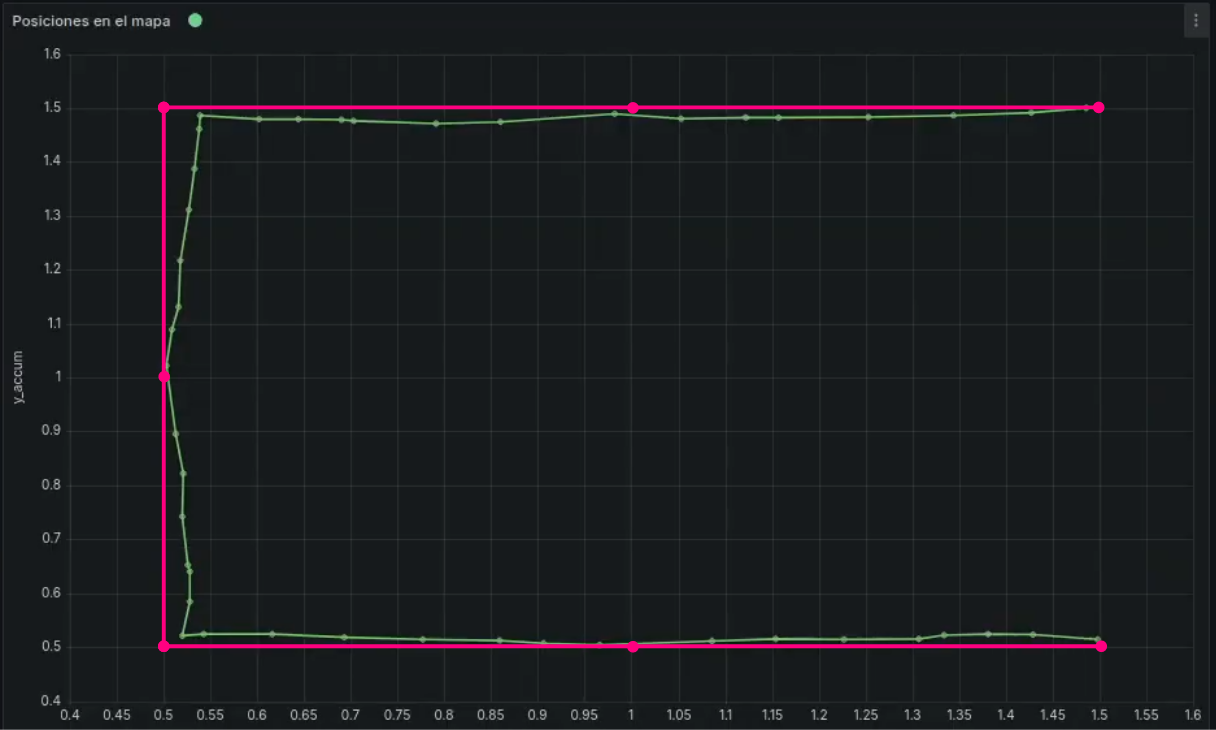
\includegraphics[width=1\linewidth]{images/ejemplo_trayectoria_compensacion_kalman.png}
    \caption{Ejemplo de una trayectoria realizada con el Filtro de Kalman}
    \label{fig:ejemplofiltrokalman}
\end{figure}

Sin embargo, durante las pruebas se identificó que el Filtro de Kalman, al estar implementado en la interfaz de Python, necesita operar a través de la red con un intercambio constante de información con el robot mediante MQTT, generando un cuello de botella en el sistema. A futuro, se considera como una mejora significativa trasladar la ejecución del Filtro de Kalman directamente al robot, eliminando la dependencia de la comunicación por red para la compensación de vectores y distancia.

\subsection{Riesgos superados}
El desarrollo de la presente iteración se corresponde con unas de las mas importantes del proyecto dado que termina de superar riesgos importantes como ser RI-04 y RI-03.

Al mismo tiempo, se logra una integración efectiva entre los nuevos y ya existentes componentes, por lo que se logran progresos sobre el riesgo RI-02.

\begin{center} \begin{tabular}{|c|c|} 
    \hline
        ID & Riesgo \\
    \hline
        RI-02 & Intercomunicación de componentes ineficiente o ineficaz \\
    \hline
        RI-03 & Prestaciones insuficientes de componentes \\
    \hline
        RI-04 & Modificación de los requerimientos del proyecto \\
    \hline
\end{tabular} \end{center}

\subsection{Conclusiones}
En esta iteración del proyecto, se alcanzaron importantes avances que fortalecen tanto la precisión como la estabilidad del sistema de control del robot omnidireccional. La implementación del Filtro de Kalman y proceso de compensación en base a él ha demostrado ser fundamental para mejorar las trayectorias y reducir los errores en el desplazamiento del robot.